\documentclass[a4paper,fleqn]{cas-sc}

\usepackage[authoryear]{natbib}

\usepackage{amsmath,amssymb,mathtools}
\usepackage{bm}

\usepackage{subcaption}
\usepackage{booktabs}
\usepackage{multirow}
\usepackage{siunitx}
\usepackage{xcolor}

\usepackage{tikz}
\usetikzlibrary{shapes.geometric, arrows.meta, positioning, calc}

\usepackage[capitalize,nameinlink,noabbrev]{cleveref}

\usepackage{lineno}
\linenumbers

\newcommand{\Kzero}{\ensuremath{K_0}}
\newcommand{\Zm}{\ensuremath{Z_m}}
\newcommand{\Vs}{\ensuremath{V_s}}
\newcommand{\ru}{\ensuremath{r_u}}
\newcommand{\pmean}{\ensuremath{p^\prime}}
\newcommand{\safeincludegraphics}[2][]{\IfFileExists{#2}{\includegraphics[#1]{#2}}{\IfFileExists{figures/#2}{\includegraphics[#1]{#2}}{\fcolorbox{gray}{white}{\begin{minipage}[c][0.22\textheight][c]{0.95\linewidth}
          \centering
          \textbf{Missing figure}\\
          \texttt{\detokenize{#2}}
        \end{minipage}
      }}}}

\graphicspath{{figures/}}

\begin{document}
\let\WriteBookmarks\relax
\def\floatpagepagefraction{1}
\def\textpagefraction{.001}

\shorttitle{Stress anisotropy effects on liquefaction resistance: DEM-HCA study}
\shortauthors{Y.~Han et~al.}

\title[mode=title]{Influence of Initial Stress Anisotropy on Liquefaction Resistance
  in Undrained Cyclic Torsional Shear: DEM Simulation of Hollow Cylinder Tests}

\author[1]{Yusong Han}
\cormark[1]
\ead{han.yusong.25z@st.kyoto-u.ac.jp}
\credit{Conceptualization, Methodology, Software, Visualization, Writing -- Original draft}

\author[2]{Ryosuke Uzuoka}
\credit{Supervision, Writing -- Review \& Editing, Funding acquisition}

\author[3]{Manta Nakamura}
\credit{Methodology, Software}

\author[2]{Kyohei Ueda}
\credit{Supervision, Writing -- Review \& Editing, Funding acquisition}

\affiliation[1]{organization={Graduate School of Engineering, Kyoto University},
            addressline={Gokasho},
            city={Uji, Kyoto},
            postcode={611-0011},
            country={Japan}}

\affiliation[2]{organization={Disaster Prevention Research Institute, Kyoto University},
            addressline={Gokasho},
            city={Uji, Kyoto},
            postcode={611-0011},
            country={Japan}}

\affiliation[3]{organization={MAEDA Corporation},
            addressline={Fujimi, Chiyoda-ku},
            city={Tokyo},
            postcode={102-8151},
            country={Japan}}

\cortext[cor1]{Corresponding author}

\begin{abstract}
The influence of initial stress anisotropy on liquefaction resistance was investigated using three-dimensional discrete element method (DEM) simulations of undrained cyclic torsional shear in hollow cylindrical specimens. A coupled analytical servo mechanism was developed in which the servo coefficients are derived from a volume-constrained stiffness matrix that accounts for the cross-coupling between radial and axial wall movements, enabling direct reproduction of laboratory hollow cylinder apparatus (HCA) boundary conditions. The investigation proceeded in two stages. First, specimens at a dense state were consolidated to a mean effective stress of 100~kPa at three representative lateral-to-vertical effective stress ratios (\Kzero{} = 0.5, 1.0, and 2.0) and subjected to cyclic loading across multiple cyclic stress ratios. The results show that liquefaction resistance exhibits a clear directional dependency: compression-state specimens (\Kzero{} = 0.5) require the most loading cycles to liquefy, isotropic specimens (\Kzero{} = 1.0) show intermediate resistance, and extension-state specimens (\Kzero{} = 2.0) liquefy fastest. Macroscopic analysis reveals that the three \Kzero{} states exhibit distinct shear-wave velocity degradation trajectories, with the compression-state specimen maintaining higher stiffness for longer, which explains the observed resistance ordering. Second, the investigation was expanded to combinations of two relative densities and five \Kzero{} values (0.5, 0.67, 1.0, 1.5, and 2.0), yielding ten cases to separate the respective roles of relative density and stress anisotropy. Microscopic analysis demonstrates that, while the mechanical coordination number primarily reflects packing compactness, the signed fabric anisotropy indicator correlates more directly with the variation in liquefaction resistance among different \Kzero{} states. Decomposition of the fabric tensor in the cylindrical coordinate system shows that contacts whose normals lie on the $z$--$\theta$ plane (the plane on which the torsional shear stress acts) directly resist torsional shear, and compression-state consolidation concentrates a larger fraction of contacts onto this plane. Contact-density distributions and force-chain visualizations further show that initially distinct fabric morphologies progressively converge toward a common dynamic equilibrium in the post-liquefaction stage, regardless of the initial stress anisotropy.
\end{abstract}

\begin{keywords}
Liquefaction resistance \sep Stress anisotropy \sep Hollow cylinder apparatus \sep
Discrete element method \sep Fabric anisotropy
\end{keywords}

\maketitle

\section{Introduction}
\label{sec:introduction}

During earthquake loading, saturated granular soils can experience a rapid rise in pore pressure that drastically reduces their shear strength. This phenomenon, termed liquefaction, has caused severe damage to infrastructure and buildings \citep{IshiharaKoga1981,SeedIdriss1967}. A large body of laboratory work has investigated liquefaction resistance using cyclic undrained triaxial tests, examining the effects of cyclic stress ratio (CSR), relative density, and confining pressure \citep{Hyodo1991,SeedLee1966,Silver1976,Toki1986}. However, vertically propagating shear waves in the ground induce gradually varying shear stress on soil elements, leading to continuous rotation of principal stress axes \citep{Arthur1980,IshiharaTowhata1983}, which cannot be fully represented in conventional triaxial loading.

Hollow cylinder apparatus (HCA) and hollow torsional shear tests address this limitation by allowing torsional loading with principal stress axis rotation. Early studies using HCA-type devices \citep[e.g.,][]{IshiharaYasuda1975,Tatsuoka1986,YamashitaToki1993} showed that liquefaction behavior can differ from triaxial-test results and depends on the loading mode and stress path. These observations motivate the use of HCA-type boundary conditions when investigating liquefaction mechanisms under more realistic cyclic loading paths.

The influence of the initial lateral-to-vertical effective stress ratio, \Kzero{}, on liquefaction resistance has been investigated extensively, yet the reported findings vary considerably depending on test conditions. Some experimental studies reported weak or negligible dependence of liquefaction strength on the initial anisotropic stress state \citep[e.g.,][]{IshiharaTakatsu1979,YamashitaToki1993}, whereas others found clear differences between isotropically consolidated (IC) and anisotropically consolidated (AC) specimens, with the trend depending on density \citep{GeorgiannouKonstadinou2014}. \citet{Vargas2020} observed that specimens under compressive consolidation exhibited higher liquefaction resistance than those consolidated isotropically. More recently, \citet{Zhao2024} conducted systematic torsional shear tests covering both compressional and extensional consolidation states and attributed the higher liquefaction resistance under compressive consolidation to smaller principal stress axis rotation during cyclic loading. While these findings establish the macroscopic trend convincingly, the particle-scale mechanisms through which stress anisotropy alters liquefaction resistance remain to be explored.

The discrete element method \citep[DEM;][]{Cundall1979} is well suited for this problem because it provides direct access to particle-scale quantities such as contact topology, force chains, and fabric anisotropy, while avoiding some specimen-to-specimen variability associated with laboratory preparation. Numerous DEM studies have examined liquefaction-related behavior in triaxial, simple-shear, or polyhedral specimen settings \citep[e.g.,][]{Huang2018,Yang2021,Jiang2021,Morimoto2021,WuYang2022,Xie2023,YangHuang2023,Zhang2023} and have identified important microscopic factors governing liquefaction resistance. Recent DEM investigations have also addressed \Kzero{} effects: \citet{YangTaiebat2024} found that both preparation protocols and \Kzero{} influence liquefaction resistance, with the difference between IC and AC states narrowing at higher densities; \citet{Otsubo2022} showed that specimens with stronger inherent anisotropy exhibit weaker stiffness in the minor principal direction and correspondingly lower liquefaction resistance. However, triaxial configurations do not incorporate principal stress axis rotation, while periodic-boundary and polyhedral specimen settings, though capable of applying general stress paths, lack direct counterparts in standard laboratory apparatus. Although DEM replication of HCA tests has precedents under drained loading \citep[e.g.,][]{Li2014,Liu2021}, extension to undrained cyclic loading in HCA geometry remains limited.

\citet{Han2024jgs} first realized undrained cyclic torsional shear in a DEM-based HCA model by introducing a combined servo mechanism that simultaneously satisfies the HCA stress boundary conditions and the constant-volume constraint. However, their formulation assumed a constant specimen height throughout, precluding axial loading and height variation, which are commonly employed loading modes in HCA tests. \citet{Ma2024} subsequently generalized this framework to accommodate a broader range of loading conditions, including drained stress paths and combined axial--torsional loading. While these formulations successfully reproduced a variety of target stress paths, three aspects of the undrained servo problem deserve closer examination.
(a)~Under undrained loading, the constant-volume constraint is a governing equation, not an auxiliary condition. It must be substituted into the kinematic system to eliminate one degree of freedom before the stress boundary conditions can form a closed system.
(b)~The servo conditions should reproduce the laboratory total-stress boundary conditions. Because the pore water pressure $u$ is a measured response rather than a prescribed input, directly targeting individual effective stresses, as in previous formulations, is only an approximation. A valid formulation must express the servo conditions in a form that does not require $u$ as an input.
(c)~Under the constant-volume constraint, the kinematic degrees of freedom (inner radius, outer radius, and height) are geometrically coupled, so movement of one wall inevitably affects the stresses on others. The servo coefficients must therefore account for this cross-coupling, rather than being derived independently from the contact stiffness at each wall.
The present study makes this closure explicit and derives closed-form servo coefficients at every timestep by analytically inverting the coupled stiffness matrix. This analytical exactness is especially important near liquefaction, where rapid loss of particle contacts causes large timestep-to-timestep stiffness changes and accumulated servo error can compromise boundary-condition control---an instability regime also noted by \citet{Ma2024}. The formulation is then applied to systematically investigate \Kzero{} effects under undrained cyclic torsional shear with direct correspondence to laboratory HCA tests.

The present work investigates the effect of initial stress anisotropy on liquefaction resistance in DEM-simulated undrained cyclic torsional shear of hollow cylindrical specimens. The investigation is organized in two stages. First, the macroscopic \Kzero{}-dependent liquefaction resistance trend is established for representative compression, isotropic, and extension states across multiple cyclic stress ratios, accompanied by energy and stiffness analyses. Second, the parameter space is expanded to two relative densities and five \Kzero{} values, and microscopic fabric analyses in the cylindrical coordinate system are used to separate the respective roles of relative density and stress anisotropy at the particle scale.

The remainder of this paper is organized as follows. Section~\ref{sec:methodology} presents the DEM-HCA model, specimen preparation and loading protocol, calibration/validation strategy, and microscopic descriptors. Section~\ref{sec:results} reports the macroscopic and microscopic responses and discusses the mechanisms governing \Kzero{}-dependent liquefaction resistance. Section~\ref{sec:conclusions} summarizes the main findings and implications.
 \section{Methodology}
\label{sec:methodology}

\subsection{DEM simulation of hollow cylinder tests}
\label{subsec:dem_hca}

DEM simulations were performed in \textsc{PFC3D} \citep{Itasca2021} to reproduce undrained cyclic torsional shear in an HCA. Unlike periodic-cell element tests, the present HCA model uses rigid boundaries (inner and outer cylinders, top and bottom planes) and six torsional blades to apply shear while preserving laboratory-relevant boundary conditions.

The specimen geometry (Fig.~\ref{fig:specimen_generation}) follows a laboratory-scale HCA configuration with inner diameter \SI{6}{cm}, outer diameter \SI{10}{cm}, and specimen height \SI{10}{cm} \citep{Vargas2020}. A rolling-resistance contact model \citep{IwashitaOda1998,WensrichKatterfeld2012} is adopted to capture non-spherical grain effects, with a particle size distribution in the range of \SIrange{1.0}{3.0}{mm}, which is a 10$\times$ scaled-up analogue of the grain size distribution of Toyoura sand. The DEM parameters are summarized in Table~\ref{tab:dem_parameters}. Particles are generated by gravity deposition from the upper part of the apparatus. Gravity is then removed to ensure a uniform stress state, and six vertically arranged torsional blades are inserted into the specimen (Fig.~\ref{fig:specimen_generation}b). Compared with the conventional approach of constraining boundary particles to transmit torque \citep[e.g.,][]{Li2014,Liu2021}, these independent wall-based blades avoid interference with the radial expansion or contraction of the cylinders, thereby preserving accurate radial stress measurement.

\begin{table}[t]
  \centering
  \caption{Parameters in DEM simulation.}
  \label{tab:dem_parameters}
  \begin{tabular}{@{}lr@{}}
    \toprule
    Description & Value \\
    \midrule
    Number of particles, $N_p$                          & 53{,}764 \\
    Particle density, $\rho_s$ (\si{kg/m^3})            & 2650 \\
    Young's modulus, $E$ (\si{GPa})                     & 0.3 \\
    Normal-to-shear stiffness ratio, $\kappa$           & 2.0 \\
    Interparticle friction, $\mu_{pp}$                  & 0.0\textsuperscript{a}\,/\,0.50\textsuperscript{b} \\
    Particle--wall friction, $\mu_{pw}$                 & 0.0 \\
    Normal critical damping ratio, $\beta_n$            & 0.7 \\
    Shear critical damping ratio, $\beta_s$             & 0.5 \\
    Rolling friction coefficient, $\mu_r$               & 0.1 \\
    \bottomrule
    \multicolumn{2}{@{}l}{\footnotesize \textsuperscript{a}Isotropic consolidation stage.} \\
    \multicolumn{2}{@{}l}{\footnotesize \textsuperscript{b}Anisotropic consolidation and cyclic shear stages.}
  \end{tabular}
\end{table}

\begin{figure*}[t]
  \centering
  \begin{tikzpicture}
\node[anchor=north west, inner sep=0] (imgA) at (0,0)
      {\includegraphics[height=5.5cm]{specimen_generation_deposit.png}};
    \node[font=\small\bfseries, anchor=north west] at
      ([xshift=4pt,yshift=-4pt]imgA.north west) {(a)};
\node[anchor=north west, inner sep=0] (imgB) at ([xshift=6pt]imgA.north east)
      {\includegraphics[height=5.5cm]{specimen_generation_postinsert.png}};
    \node[font=\small\bfseries, anchor=north west] at
      ([xshift=4pt,yshift=-4pt]imgB.north west) {(b)};
\node[anchor=north west, inner sep=0] (cbar) at ([xshift=6pt]imgB.north east)
      {\includegraphics[height=5.5cm]{colorbar_viridis.png}};
\foreach \val/\frc in {1.5/0, 1.25/0.25, 1.0/0.5, 0.75/0.75, 0.5/1.0} {
      \node[font=\footnotesize, anchor=west] at
        ([xshift=2pt, yshift={-\frc*5.5cm}]cbar.north east) {\val};
    }
\node[font=\footnotesize, rotate=90, anchor=south] at
      ([xshift=40pt]cbar.east) {Particle radius (mm)};
  \end{tikzpicture}
  \caption{Initial specimen generation process in the DEM-based hollow cylinder apparatus model.
    Particles are colored by radius.
    (a)~Particle generation modeling air-pluviation.
    (b)~Insertion of torsional blades.}
  \label{fig:specimen_generation}
\end{figure*}

The stress and strain evaluation expressions for the HCA geometry are summarized in Appendix~\ref{sec:appendix_hca}.

\subsection{Specimen preparation and anisotropic consolidation protocol}
\label{subsec:preparation}

Specimens are prepared using an isotropic-consolidation to anisotropic-consolidation (IC--AC) protocol. First, the assembly is compressed under zero interparticle friction to a target void ratio, which is determined through the iterative calibration procedure described in Section~\ref{subsec:calibration_validation}: approximately 0.736 for the dense state ($D_r \approx 90\%$) and 0.742 for the medium-dense state ($D_r \approx 75\%$). The interparticle friction coefficient is then restored to 0.5, and the specimen is consolidated from an isotropic state (\Kzero{} = 1.0, $\pmean=\SI{10}{kPa}$) to the target mean effective stress ($\pmean=\SI{100}{kPa}$) along a linear anisotropic stress path.

During the AC stage, $\pmean$ is increased from \SI{10}{kPa} to \SI{100}{kPa} through ten equally spaced target stress states along a linear anisotropic stress path. The resulting stress paths and void-ratio evolution for the three primary cases are shown in Fig.~\ref{fig:ac_path}. The markers in Fig.~\ref{fig:ac_path_a} correspond to the prescribed target states; the solid lines between them represent the actual stress evolution, which exhibits minor fluctuations that arise because different \Kzero{} states require different amounts of axial strain to reach the same $\pmean$ increment---compression-state specimens (\Kzero{} = 0.5) undergo larger axial strain per step, causing the axial stress to lag slightly behind the radial stress during each increment. These fluctuations vanish at each target state, confirming that the servo accurately satisfies the prescribed stress conditions. The final void ratio differs only slightly among the three states (on the order of $10^{-3}$), which allows the comparison to focus on fabric-related effects rather than void-ratio differences. Figure~\ref{fig:ac_specimens} shows the three specimens after consolidation, with force-chain networks and particle arrangements displayed side by side; the visual contrast in force-chain directionality reflects the different \Kzero{} states.

\begin{figure}[t]
  \centering
  \begin{subfigure}[t]{0.432\linewidth}
    \centering
    \safeincludegraphics[width=\linewidth]{anisotropic_consolidation_stress_path.png}
    \caption{$\pmean$--$q$ stress path.}
    \label{fig:ac_path_a}
  \end{subfigure}
  \hfill
  \begin{subfigure}[t]{0.432\linewidth}
    \centering
    \safeincludegraphics[width=\linewidth]{anisotropic_consolidation_void_ratio.png}
    \caption{$\pmean$--$e$ evolution.}
    \label{fig:ac_path_b}
  \end{subfigure}
  \caption{Stress and void-ratio evolution during anisotropic consolidation for the three representative \Kzero{} states.}
  \label{fig:ac_path}
\end{figure}

\begin{figure*}[t]
  \centering
  \begin{tikzpicture}
\node[anchor=north west, inner sep=0] (imgA) at (0,0)
      {\includegraphics[height=4.8cm]{specimen_k0_05_after_ac.png}};
    \node[font=\small, anchor=north] at (imgA.south) {(a) \Kzero{} = 0.5};
\node[anchor=north west, inner sep=0] (imgB) at ([xshift=3pt]imgA.north east)
      {\includegraphics[height=4.8cm]{specimen_k0_10_after_ac.png}};
    \node[font=\small, anchor=north] at (imgB.south) {(b) \Kzero{} = 1.0};
\node[anchor=north west, inner sep=0] (imgC) at ([xshift=3pt]imgB.north east)
      {\includegraphics[height=4.8cm]{specimen_k0_20_after_ac.png}};
    \node[font=\small, anchor=north] at (imgC.south) {(c) \Kzero{} = 2.0};
\node[anchor=north west, inner sep=0] (cbar) at ([xshift=3pt]imgC.north east)
      {\includegraphics[height=4.8cm]{colorbar_viridis_force.png}};
\foreach \val/\frc in {2.0/0, 1.5/0.25, 1.0/0.5, 0.5/0.75, 0/1.0} {
      \node[font=\footnotesize, anchor=west] at
        ([xshift=2pt, yshift={-\frc*4.8cm}]cbar.north east) {\val};
    }
\node[font=\footnotesize, rotate=90, anchor=south] at
      ([xshift=34pt]cbar.east) {Contact force magnitude (N)};
  \end{tikzpicture}
  \caption{DEM HCA specimens after anisotropic consolidation to $\pmean=\SI{100}{kPa}$.
    The left half of each panel shows interparticle force chains colored by contact force magnitude.}
  \label{fig:ac_specimens}
\end{figure*}

The cyclic shear simulation program consists of two sets. In the primary set, three representative \Kzero{} states---0.5 (compression), 1.0 (isotropic), and 2.0 (extension)---are examined at a dense state ($D_r \approx 90\%$) across multiple CSR levels to characterize how liquefaction resistance varies with the direction and magnitude of stress anisotropy, and to trace the associated energy dissipation, stiffness degradation, and fabric evolution. In the expanded set, a medium-dense state ($D_r \approx 75\%$) is introduced alongside the dense state, and two additional \Kzero{} values (0.67 and 1.5) are included to refine the coverage of anisotropy levels, yielding ten cases ($2 \times 5$) at a single CSR = 0.300. This expanded set allows examination of whether the \Kzero{}-dependent liquefaction resistance trend observed at $D_r \approx 90\%$ persists at a lower density, and provides a broader parametric basis for the subsequent microscopic analysis.

\subsection{Undrained cyclic torsional shear loading}
\label{subsec:cyclic_loading}

\begin{figure*}[t]
  \centering
  \includegraphics[width=\textwidth]{fig_hca_standalone.pdf}
  \caption{Schematic of the hollow cylinder apparatus (HCA) specimen.
    The left half of each panel shows the laboratory boundary conditions with total stresses
    ($p_o$, $p_i$, $p_z$);
    the right half shows the DEM representation with effective stresses
    ($p_o^\prime$, $p_i^\prime$, $p_z^\prime$).
    (a)~Perspective view with specimen height $H$.
    (b)~Plan view showing the annular geometry with inner radius $r$,
    outer radius $R$, and torque $T$.}
  \label{fig:hca_schematic}
\end{figure*}

In a laboratory HCA (left half of Fig.~\ref{fig:hca_schematic}), the specimen is enclosed between an outer chamber (pressure $p_o$) and an inner chamber (pressure $p_i$), which are controlled independently. An axial load is applied through the loading piston, producing a vertical pressure $p_z$, and a torque $T$ is transmitted through end platens. Under undrained conditions the pore water pressure $u$, monitored by pressure transducers, is uniform throughout the specimen, so the effective pressures are $p_o^{\prime}=p_o-u$, $p_i^{\prime}=p_i-u$, and $p_z^{\prime}=p_z-u$. Because $u$ drops out in any difference of effective pressures, the radial pressure difference equals its total-stress counterpart, $p_o^{\prime}-p_i^{\prime}=p_o-p_i$, and so does the axial pressure difference between the vertical and average radial effective stresses (Table~\ref{tab:hca_equations}): $p_z^{\prime}-\sigma_r^{\prime}=p_z-\sigma_r$.

The constant-volume method is a well-established approach in DEM for reproducing undrained cyclic loading \citep{YimsiriSoga2010}. In this method, the pore water pressure is not modelled explicitly; instead, the contact forces between particles and walls yield effective stresses ($p_o^{\prime}$, $p_i^{\prime}$, $p_z^{\prime}$; right half of Fig.~\ref{fig:hca_schematic}) directly (Table~\ref{tab:hca_equations}). The DEM-based HCA specimen has four kinematic degrees of freedom---inner radius rate ($dr/dt$), outer radius rate ($dR/dt$), height rate ($dH/dt$), and rotation angle rate ($d\theta/dt$), where $r$ is the inner radius, $R$ the outer radius (Fig.~\ref{fig:hca_schematic}b), and $H$ the height of the hollow cylindrical specimen (Fig.~\ref{fig:hca_schematic}a)---and the following laboratory boundary conditions to reproduce: the undrained (constant-volume) constraint, the inner and outer cell pressures, the axial stress, and the torsional shear stress.

Among these, the constant-volume constraint provides one equation linking $dr/dt$, $dR/dt$, and $dH/dt$, while the torsional condition is satisfied by adjusting the rotation rate $d\theta/dt$ to match the target torque. The remaining challenge is to map the three effective pressures accessible in DEM---$p_i^{\prime}$, $p_o^{\prime}$, and $p_z^{\prime}$---to the laboratory total-stress boundary conditions, where the unknown pore water pressure $u$ prevents a direct one-to-one correspondence. The difference relations established above resolve this difficulty: because $u$ drops out, the two differences $p_o^{\prime}-p_i^{\prime}=p_o-p_i$ and $p_z^{\prime}-\sigma_r^{\prime}=p_z-\sigma_r$ map the DEM effective stresses to the laboratory total-stress conditions without requiring $u$, yielding two independent equations that, together with the volume constraint and the torsional condition, close the system of four equations for four unknowns.

\paragraph{Radial condition.}
The radial condition controls the pressure difference between the outer and inner cylinders. The radial pressure difference and its servo error are defined as:
\begin{equation}
p_{dif,r}^{\prime} = p_o^{\prime} - p_i^{\prime}, \qquad e_r = p_{dif,r}^{\prime} - p_{dif,r}^{tar},
\label{eq:cond1_radial}
\end{equation}
where $p_o^{\prime}$ and $p_i^{\prime}$ are the outer and inner radial effective pressures (Table~\ref{tab:hca_equations}) and $p_{dif,r}^{tar}$ is the target radial pressure difference. The servo must drive $e_r$ to zero at each timestep to satisfy this condition.

\paragraph{Axial condition.}
Laboratory HCA tests can operate under either constant total axial stress or constant specimen height.
(i)~\emph{Stress-control mode}: the servo controls the difference between the vertical and radial effective stresses, analogous to the radial condition in \cref{eq:cond1_radial}. The axial pressure difference and its servo error are defined as:
\begin{equation}
p_{dif,z}^{\prime} = p_z^{\prime} - \sigma_r^{\prime}, \qquad e_z = p_{dif,z}^{\prime} - p_{dif,z}^{tar},
\label{eq:cond2_axial}
\end{equation}
where $p_z^{\prime}$ is the vertical effective pressure (Table~\ref{tab:hca_equations}), $\sigma_r^{\prime}$ is the average radial effective stress, and $p_{dif,z}^{tar}$ is the target axial pressure difference. The servo must drive $e_z$ to zero at each timestep to satisfy this condition.
(ii)~\emph{Displacement-control mode}: the specimen height is held constant ($dH/dt=0$), and $p_{dif,z}^{\prime}$ evolves freely.

\paragraph{Torsional condition.}
The torque error is defined as:
\begin{equation}
e_T = T - T^{tar},
\label{eq:cond3_torsion_error}
\end{equation}
where $T$ is the current torque and $T^{tar}$ is the target torque. The servo must drive $e_T$ to zero at each timestep to satisfy the prescribed torsional loading.

\paragraph{Volume constraint.}
The undrained (constant-volume) condition requires (with the outward-positive sign convention $dr>0$, $dR>0$ denoting radius increases):
\begin{equation}
2\pi H\!\left(R\frac{dR}{dt} - r\frac{dr}{dt}\right) + \pi\!\left(R^2-r^2\right)\frac{dH}{dt} = 0.
\label{eq:const_volume_constraint}
\end{equation}

\paragraph{Analytical servo.}
The four conditions above---radial (\cref{eq:cond1_radial}), axial (\cref{eq:cond2_axial}), torsional (\cref{eq:cond3_torsion_error}), and constant-volume (\cref{eq:const_volume_constraint})---provide four independent equations for the four kinematic unknowns ($dr/dt$, $dR/dt$, $dH/dt$, $d\theta/dt$). The system is therefore closed and can be solved analytically.

An analytical solution is obtained by reducing the four unknowns to two through two successive eliminations:
\begin{enumerate}
\item \emph{Torsion.} The torsional condition (\cref{eq:cond3_torsion_error}) does not enter the kinematic constraints that govern $dr/dt$, $dR/dt$, and $dH/dt$. It is therefore solved independently at each timestep by adjusting the rotation angle rate:
\begin{equation}
\frac{d\theta}{dt} = \frac{e_T}{\Delta t}\,S_T,
\label{eq:cond3_torsion}
\end{equation}
where $\Delta t$ is the simulation timestep and $S_T$ is the torsional servo coefficient, determined from the contact-stiffness-weighted rotational stiffness $I_{rot}$ about the specimen axis (Fig.~\ref{fig:servo_geometry}):
\begin{equation}
I_{rot} = \sum k_n\bigl[(\mathbf{r}_d\times\hat{\mathbf{z}})\cdot\mathbf{n}\bigr]^2, \qquad S_T = \frac{1}{I_{rot}},
\label{eq:irot_scs}
\end{equation}
where $\mathbf{r}_d$ is the position vector from the rotation axis to the contact point in the horizontal plane, $\hat{\mathbf{z}}$ is the unit vector along the specimen axis, $\mathbf{n}$ is the contact normal directed from the particle centre to the blade, and $k_n$ is the normal contact stiffness.

\begin{figure}[t]
  \centering
  \begin{tikzpicture}[
    every node/.style={font=\small},
    lbl/.style={font=\footnotesize},
    dimarr/.style={{Stealth[length=3pt]}-{Stealth[length=3pt]}, thin, black},
  ]
    \node[anchor=south west, inner sep=0] (img) at (0,0)
      {\includegraphics[width=0.5\linewidth]{servo_torsional_contact_geometry.png}};
    \begin{scope}[
      x={(img.south east)},
      y={(img.north west)},
    ]
      \coordinate (CP) at (0.646, 0.276);
      \coordinate (RA) at (0.4, 0.80);
      \coordinate (RA_h) at (0.4, 0.56);

      \node[lbl, red!70!black, above right] at (0.46, 0.4) {$\mathbf{n}$};

      \draw[-{Stealth[length=3pt]}, thick, blue!70!black] (RA_h) -- (CP);
      \node[lbl, blue!70!black, above] at ($(RA_h)!0.52!(CP)$) {$\mathbf{r}_d$};
      \draw[-{Stealth[length=3pt]}, thick, black] (RA_h) -- (RA);
      \node[lbl, black, right] at ($(RA_h)!0.7!(RA)$) {$\hat{\mathbf{z}}$};
    \end{scope}
  \end{tikzpicture}
  \caption{Contact geometry used to evaluate the rotational stiffness contribution for torsional servo control. $\mathbf{r}_d$: position vector from the rotation axis to the contact point in the horizontal plane; $\mathbf{n}$: contact normal directed from particle centre to blade; $\hat{\mathbf{z}}$: unit vector along the specimen axis.}
  \label{fig:servo_geometry}
\end{figure}
\item \emph{Volume constraint.} \Cref{eq:const_volume_constraint} expresses $dR/dt$ as a function of $dr/dt$ and $dH/dt$, reducing the system to two unknowns ($dr/dt$, $dH/dt$) with two target conditions ($e_r=0$ and $e_z=0$ in \cref{eq:cond1_radial,eq:cond2_axial}).
\end{enumerate}

After these two eliminations, both the radial and axial conditions depend on the same two unknowns ($dr/dt$, $dH/dt$). Because the volume constraint expresses $dR/dt$ as a function of $dr/dt$ and $dH/dt$, the outer-cylinder pressure $p_o^{\prime}$ is no longer independent: the radial condition, which involves both $p_i^{\prime}$ and $p_o^{\prime}$, is therefore affected by both $dr/dt$ and $dH/dt$ simultaneously. Similarly, the axial condition involves $p_z^{\prime}$ (affected by $dH/dt$) and $\sigma_r^{\prime}=({p_o^{\prime}R+p_i^{\prime}r})/({R+r})$ (Table~\ref{tab:hca_equations}), which depends on both cylinder movements. The two conditions are thus fully coupled. The next step is to quantify the contributions of $dr/dt$ and $dH/dt$ to the stress increments on all three walls, from which the coupled servo coefficients can be derived.

Let $K_{r,i}$ and $K_{r,o}$ denote the aggregate normal contact stiffness at the inner and outer cylinders, $A_i=2\pi rH$ and $A_o=2\pi RH$ the corresponding wall areas, and $K_z=\frac{1}{2}\sum_{c\in\mathrm{top/bottom}} k_n$ the effective axial contact stiffness with area $A_z=2\pi(R^2-r^2)$. Substituting \cref{eq:const_volume_constraint} into the pressure increments yields the coupled stiffness relation (derived in Appendix~\ref{sec:appendix_servo}):
\begin{equation}
\begin{pmatrix} \delta p_{dif,r}^{\prime} \\[4pt] \delta p_{dif,z}^{\prime} \end{pmatrix}
=
\underbrace{\begin{pmatrix} \hat{K}_{11} & \hat{K}_{12} \\[6pt] \hat{K}_{21} & \hat{K}_{22} \end{pmatrix}}_{\hat{\mathbf{K}}}
\begin{pmatrix} dr \\[4pt] dH \end{pmatrix},
\label{eq:coupled_stiffness}
\end{equation}
where
\begin{alignat}{2}
\hat{K}_{11} &= -\frac{K_{r,i}}{A_i}-\frac{r}{R}\,\frac{K_{r,o}}{A_o}, &\qquad
\hat{K}_{12} &= \frac{R^2-r^2}{2RH}\,\frac{K_{r,o}}{A_o}, \label{eq:Khat_main_row1}\\[4pt]
\hat{K}_{21} &= -\frac{K_{r,i}-\frac{r}{R}\,K_{r,o}}{A_i+A_o}, &\qquad
\hat{K}_{22} &= -\frac{K_z}{A_z}-\frac{(R^2-r^2)\,K_{r,o}}{2RH\,(A_i+A_o)}. \label{eq:Khat_main_row2}
\end{alignat}
The entries carry dimensions of Pa/m and incorporate the volume-constraint coupling. The determinant of $\hat{\mathbf{K}}$ is
\begin{equation}
\det(\hat{\mathbf{K}}) = \hat{K}_{11}\,\hat{K}_{22} - \hat{K}_{12}\,\hat{K}_{21}.
\label{eq:det_K_main}
\end{equation}
Setting $(\delta p_{dif,r}^{\prime},\,\delta p_{dif,z}^{\prime})=(-e_r,\,-e_z)$ and inverting \cref{eq:coupled_stiffness} yields the coupled servo equations:
\begin{align}
\frac{dr}{dt} &= S_{rr}\,\frac{e_r}{\Delta t} + S_{rz}\,\frac{e_z}{\Delta t}, \label{eq:servo_dr}\\[6pt]
\frac{dH}{dt} &= S_{zr}\,\frac{e_r}{\Delta t} + S_{zz}\,\frac{e_z}{\Delta t}, \label{eq:servo_dH}
\end{align}
where the servo coefficients are the entries of $\hat{\mathbf{K}}^{-1}$:
\begin{alignat}{2}
S_{rr} &= \frac{-\hat{K}_{22}}{\det(\hat{\mathbf{K}})}, &\qquad
S_{rz} &= \frac{\hat{K}_{12}}{\det(\hat{\mathbf{K}})}, \label{eq:servo_coeff_r}\\[4pt]
S_{zr} &= \frac{\hat{K}_{21}}{\det(\hat{\mathbf{K}})}, &\qquad
S_{zz} &= \frac{-\hat{K}_{11}}{\det(\hat{\mathbf{K}})}. \label{eq:servo_coeff_z}
\end{alignat}
The diagonal terms $S_{rr}$ and $S_{zz}$ represent the direct servo response, while the off-diagonal terms $S_{rz}$ and $S_{zr}$ capture the cross-coupling between the radial and axial conditions. The remaining kinematic variable $dR/dt$ is then obtained by substituting $dr/dt$ and $dH/dt$ into \cref{eq:const_volume_constraint}. The exact analytical solution of the coupled stiffness matrix ensures that the servo coefficients are physically consistent, providing the correct basis on which a relaxation factor ($<1$) can be applied for numerical stability. Under the constant specimen height condition ($dH/dt=0$) adopted by \citet{Han2024jgs}, only the radial condition remains active and the servo coefficient reduces to
\begin{equation}
S_{rr} = -\frac{1}{\hat{K}_{11}} = \frac{1}{\dfrac{K_{r,i}}{A_i}+\dfrac{r}{R}\,\dfrac{K_{r,o}}{A_o}}.
\label{eq:Srr_constantH_main}
\end{equation}

\begin{figure}[t]
  \centering
  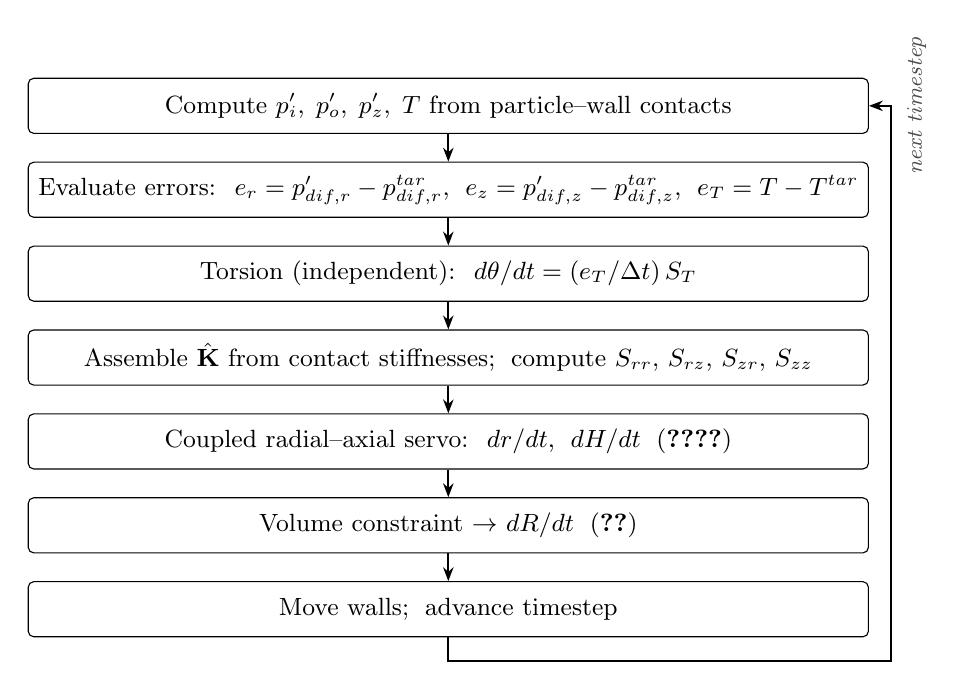
\begin{tikzpicture}[
    node distance=10pt,
    box/.style={draw, rounded corners=2pt, minimum width=0.88\linewidth,
                minimum height=7mm, align=center, font=\small},
    decision/.style={draw, diamond, aspect=2.5, minimum width=0.7\linewidth,
                     align=center, font=\small, inner sep=1pt},
    arr/.style={-{Stealth[length=5pt]}, thick},
    label/.style={font=\footnotesize\itshape, text=black!70},
  ]
    \node[box] (step1)
      {Compute $p_i^{\prime},\;p_o^{\prime},\;p_z^{\prime},\;T$
       from particle--wall contacts};
    \node[box, below=of step1] (step2)
      {Evaluate errors:\;
       $e_r=p_{dif,r}^{\prime}-p_{dif,r}^{tar}$,\;
       $e_z=p_{dif,z}^{\prime}-p_{dif,z}^{tar}$,\;
       $e_T=T-T^{tar}$};
    \node[box, below=of step2] (step3)
      {Torsion (independent):\;
       $d\theta/dt = (e_T/\Delta t)\,S_T$};
    \node[box, below=of step3] (step4)
      {Assemble $\hat{\mathbf{K}}$ from contact stiffnesses;\;
       compute $S_{rr},\,S_{rz},\,S_{zr},\,S_{zz}$};
    \node[box, below=of step4] (step5)
      {Coupled radial--axial servo:\;
       $dr/dt$,\; $dH/dt$ \;(\cref{eq:servo_dr,eq:servo_dH})};
    \node[box, below=of step5] (step6)
      {Volume constraint $\rightarrow$ $dR/dt$
       \;(\cref{eq:const_volume_constraint})};
    \node[box, below=of step6] (step7)
      {Move walls;\; advance timestep};

    \draw[arr] (step1) -- (step2);
    \draw[arr] (step2) -- (step3);
    \draw[arr] (step3) -- (step4);
    \draw[arr] (step4) -- (step5);
    \draw[arr] (step5) -- (step6);
    \draw[arr] (step6) -- (step7);
    \draw[arr] (step7.south) -- ++(0,-0.3) -| ([xshift=8pt]step1.east |- step7.south) -- ([xshift=8pt]step1.east) -- (step1.east)
      node[label, pos=0.45, right=20pt, rotate=90, anchor=south] {next timestep};
  \end{tikzpicture}
  \caption{Servo procedure at each simulation timestep during undrained loading.}
  \label{fig:servo_flowchart}
\end{figure}

The excess pore water pressure is inferred from the reduction in radial effective stress:
\begin{equation}
u = \sigma_{r0}^{\prime} - \sigma_r^{\prime},
\label{eq:epwp_definition}
\end{equation}
where $u$ is the excess pore water pressure, $\sigma_r^{\prime}$ is the current radial effective stress, and $\sigma_{r0}^{\prime}$ is its initial value. The ratio $\ru$ is then defined as $\ru = u/\sigma_{r0}^{\prime}$. Figure~\ref{fig:servo_flowchart} summarizes the complete servo procedure applied at each simulation timestep.

Compared with earlier DEM-based HCA servo strategies, the present formulation makes three contributions explicit. First, the governing equations are systematically reduced through elimination of the volume constraint and torsional independence before the coupled system is solved, clarifying the mathematical structure of the problem. Second, the laboratory-to-DEM mapping is established through two pressure differences ($p_{dif,r}^{\prime}$ and $p_{dif,z}^{\prime}$), which are the correct servo targets because they are invariant to the unknown pore water pressure. Third, the cross-coupling between the radial and axial degrees of freedom is quantified analytically through the off-diagonal entries of $\hat{\mathbf{K}}$, so that the servo coefficients correctly reflect the mutual influence of $dr/dt$ and $dH/dt$ on both boundary conditions. None of these steps were formalized in earlier work: \citet{Han2024jgs} solved only the radial and torsional conditions while keeping the specimen height fixed, thereby bypassing the axial degree of freedom entirely, and \citet{Ma2024} introduced an axial servo but derived each servo coefficient from the contact stiffness at the corresponding wall independently, without reflecting the cross-coupling among the wall movements.

\subsection{Parameter calibration and validation}
\label{subsec:calibration_validation}

The micro-parameters listed in Table~\ref{tab:dem_parameters} were calibrated against the undrained monotonic torsional shear data of \citet{Nakata1998} for dense Toyoura sand ($D_r \approx 90\%$, $\pmean_0=\SI{100}{kPa}$, \Kzero{} = 1.0) \citep[see also][]{Ma2024}. Because the micro-parameters collectively influence shear stiffness, dilatancy, and liquefaction resistance, the calibration targeted these behaviors in sequence. Starting from a base parameter set at a given void ratio, the contact Young's modulus $E$ and rolling friction coefficient $\mu_r$ were adjusted while keeping the normal-to-shear stiffness ratio $\kappa$ constant, aiming to reproduce the shear stiffness observed in the $\varepsilon_q$--$q$ response of the monotonic shear tests. The effective stress path in $\pmean$--$q$ space was then examined to assess dilatancy. If the simulated dilatancy was insufficient---i.e., the mean effective stress at phase transformation was lower than the experimental value---the specimen was further compacted to a lower void ratio, which increased both dilatancy and shear stiffness; $E$ was then reduced accordingly to restore the target shear stiffness. This iterative process between void ratio, contact modulus, and rolling friction was repeated until both the shear stiffness and dilatancy simultaneously matched the monotonic experimental data. During the monotonic calibration, the axial pressure difference was maintained at zero ($p_{dif,z}^{tar}=0$ in \cref{eq:cond2_axial}) to ensure $\sigma_z^{\prime}=\sigma_r^{\prime}$ during shearing.

The calibrated parameter set was then validated against the cyclic liquefaction resistance data of \citet{Ishihara1985} for the same sand under identical conditions. Specimens were subjected to sinusoidal torsional shear at five CSR levels (0.20, 0.25, 0.30, 0.35, and 0.40) under constant specimen height ($dH/dt=0$), matching the experimental protocol of \citet{Ishihara1985}, with liquefaction defined by single-amplitude shear strain $\gamma_{SA}=2.5\%$.

\begin{figure*}[t]
  \centering
  \safeincludegraphics[width=\textwidth]{validate_combined.png}
  \caption{Calibration and validation of the DEM-HCA model for dense Toyoura sand ($D_r \approx 90\%$, $\pmean_0=\SI{100}{kPa}$, \Kzero{} = 1.0): (a) effective stress path and (b) stress--strain relationship from undrained monotonic shear, calibrated against \citet{Nakata1998}; (c) cyclic stress ratio versus number of cycles to liquefaction, validated against \citet{Ishihara1985}.}
  \label{fig:validation_combined}
\end{figure*}

Fig.~\ref{fig:validation_combined} summarizes the calibration and validation results. The effective stress path (Fig.~\ref{fig:validation_combined}a) captures the initial contraction followed by dilation towards the critical state line, matching the experimental trend. The stress--strain relationship (Fig.~\ref{fig:validation_combined}b) reproduces the shear stiffness and strain-hardening behavior. These two aspects confirm a successful calibration against the monotonic data. The liquefaction resistance curve (Fig.~\ref{fig:validation_combined}c) shows good agreement with the cyclic data across the full range of CSR, validating the calibrated parameters under cyclic loading conditions without further adjustment. The simultaneous agreement across stiffness, dilatancy, and cyclic liquefaction resistance confirms the reliability of the micro-parameters (Table~\ref{tab:dem_parameters}) and demonstrates that the servo mechanism performs well under both axial stress-control (monotonic calibration) and displacement-control (cyclic validation) modes.

\subsection{Microscopic descriptors}
\label{subsec:micro_descriptors}

While the macroscopic response characterizes the overall liquefaction behavior, a key advantage of DEM is its ability to access particle-scale information that is not directly measurable in laboratory tests. To exploit this advantage, three microscopic descriptors are introduced to probe the contact network from complementary perspectives: the mechanical coordination number \Zm{}, the signed fabric anisotropy indicator $\alpha$, and the contact density $\rho_c$.

The mechanical coordination number \citep{Thornton2000,Oda1977} is defined as
\begin{equation}
Z_m = \frac{2N_c - N_1}{N_p - N_1 - N_0},
\label{eq:zm_definition_method}
\end{equation}
where $N_c$ is the total number of interparticle contacts, $N_p$ is the total number of particles, and $N_1$ and $N_0$ are the numbers of particles with one and zero contacts, respectively. Floaters are excluded to focus on the load-bearing contact network. $Z_m$ serves as a scalar measure of packing compactness.

The directionality of the contact network is characterized through the fabric tensor \citep{Oda1982fabric,Oda1982stat}:
\begin{equation}
\Phi_{ij} = \frac{1}{N_c}\sum n_i\,n_j,
\label{eq:fabric_tensor}
\end{equation}
where $n_i$ and $n_j$ are the components of the contact normal vector. Because the HCA specimen is axisymmetric about the vertical axis $z$, it is natural to express $\Phi_{ij}$ in the cylindrical coordinate system $(r,\theta,z)$. The signed scalar indicator $\alpha$ \citep{YimsiriSoga2010,Otsubo2022} is then defined from the axial diagonal component $\Phi_{zz}$:
\begin{equation}
\alpha = \frac{5(3\Phi_{zz} - 1)}{5\Phi_{zz} + 1}.
\label{eq:alpha_definition_method}
\end{equation}
Positive $\alpha$ indicates that contact normals concentrate toward the vertical axis (compression-state anisotropy, \Kzero{} $< 1.0$), whereas negative $\alpha$ indicates concentration toward the horizontal plane (extension-state anisotropy, \Kzero{} $> 1.0$).

The contact density \citep{Han2023} describes the average number of contacts per unit solid angle on the unit sphere of contact normal orientations:
\begin{equation}
\rho_c(\theta_z,\,\phi_{\mathrm{cir}}) = \frac{2\,N(\theta_z,\,\phi_{\mathrm{cir}})}{N_p\,\Delta\Omega},
\label{eq:contact_density}
\end{equation}
where $\theta_z$ and $\phi_{\mathrm{cir}}$ are the polar and azimuthal angles in the spherical coordinate system, $N(\theta_z,\,\phi_{\mathrm{cir}})$ is the number of contacts whose normals fall within the angular bin of widths $\Delta\theta_z$ and $\Delta\phi_{\mathrm{cir}}$, and $\Delta\Omega = (\cos\phi_{\mathrm{cir}} - \cos(\phi_{\mathrm{cir}}+\Delta\phi_{\mathrm{cir}}))\,\Delta\theta_z$ is the solid angle subtended by that bin. Unlike the fabric tensor, $\rho_c$ retains the full directional information and thus provides a more complete picture of the evolving contact network.

Together, these three descriptors probe the contact network at increasing levels of directional detail: \Zm{} quantifies the average contact density per particle (scalar), $\alpha$ captures the dominant anisotropy direction (signed scalar), and $\rho_c$ resolves the full directional distribution (field on the unit sphere). They are used alongside force-chain visualizations to connect particle-scale fabric evolution to the macroscopic liquefaction resistance trends reported in \cref{sec:results}.
 \section{Results and Discussion}
\label{sec:results}

\subsection{Macroscopic response and liquefaction resistance}
\label{subsec:macro_response}

The macroscopic response is examined first to establish the overall liquefaction resistance ordering among \Kzero{} states, which then serves as the target behavior to be interpreted through energy and stiffness indicators (Section~\ref{subsec:energy_stiffness}) and microscopic fabric descriptors (Section~\ref{subsec:micro_fabric_results}). Figure~\ref{fig:macro_response} presents a combined overview of the typical macroscopic response during undrained cyclic torsional shear at CSR = 0.200.

\begin{figure*}[t]
  \centering
  \begin{subfigure}[t]{0.48\textwidth}
    \centering
    \safeincludegraphics[width=\linewidth]{macro_response_a.png}
    \caption{$\tau_{z\theta}$ vs. $\pmean$ for \Kzero{} = 1.0.}
    \label{fig:macro_response_a}
  \end{subfigure}
  \hfill
  \begin{subfigure}[t]{0.48\textwidth}
    \centering
    \safeincludegraphics[width=\linewidth]{macro_response_b.png}
    \caption{$\tau_{z\theta}$ vs. $\gamma_{z\theta}$ for \Kzero{} = 1.0.}
    \label{fig:macro_response_b}
  \end{subfigure}

  \vspace{0.5em}

  \begin{subfigure}[t]{0.48\textwidth}
    \centering
    \safeincludegraphics[width=\linewidth]{macro_response_c.png}
    \caption{Deviatoric stress vs. $\pmean$ for three \Kzero{} states.}
    \label{fig:macro_response_c}
  \end{subfigure}
  \hfill
  \begin{subfigure}[t]{0.48\textwidth}
    \centering
    \safeincludegraphics[width=\linewidth]{macro_response_d.png}
    \caption{Excess pore pressure ratio $\ru$ evolution for three \Kzero{} states.}
    \label{fig:macro_response_d}
  \end{subfigure}
  \caption{Typical macroscopic response during undrained cyclic torsional shear at a representative cyclic stress ratio.}
  \label{fig:macro_response}
\end{figure*}

As shown in Fig.~\ref{fig:macro_response}(a,\,b), the isotropically consolidated specimen (\Kzero{} = 1.0) exhibits the classical undrained cyclic response: progressive reduction in $\pmean$ with a butterfly-shaped effective stress path, and marked stiffness degradation with increasingly nonlinear hysteretic loops.

When the three \Kzero{} states are compared in Fig.~\ref{fig:macro_response}(c,\,d), their stress paths converge toward a similar low-effective-stress state near the origin, but the rate of effective stress loss differs systematically: the \Kzero{} = 2.0 specimen accumulates excess pore pressure fastest, the \Kzero{} = 0.5 specimen slowest, and the \Kzero{} = 1.0 specimen is intermediate. Initial stress anisotropy therefore governs the rate of effective stress reduction rather than the ultimate state at liquefaction. Both the stress-based ($\ru = 0.95$) and strain-based ($\gamma_{SA} = 2.5\%$) criteria yield the same ordering of the number of cycles to liquefaction $N_L$ among \Kzero{} states; the stress-based criterion is adopted hereafter.

\begin{figure}[t]
  \centering
  \safeincludegraphics[width=0.554\linewidth]{liquefaction_resistance_curves.png}
  \caption{Cyclic liquefaction resistance curves for specimens with three representative stress anisotropies (\Kzero{} = 0.5, 1.0, 2.0). The inset shows the expanded \Kzero{} set at CSR = 0.300 (\Kzero{} = 0.5, 0.67, 1.0, 1.5, 2.0) to illustrate the intermediate states.}
  \label{fig:liq_resistance_curves}
\end{figure}

To quantify the \Kzero{} effect over a range of cyclic stress ratios, the CSR--$N_L$ relationship for the three representative anisotropic states is shown in Fig.~\ref{fig:liq_resistance_curves}. Across all CSR levels, $N_L$ decreases monotonically from \Kzero{} = 0.5 through 1.0 to 2.0; the inset at CSR = 0.300, which includes two additional intermediate states (\Kzero{} = 0.67 and 1.5), confirms this trend. The effect of \Kzero{} depends on the direction of deviatoric stress: compression-type anisotropy (\Kzero{} < 1.0) enhances liquefaction resistance, while extension-type anisotropy (\Kzero{} > 1.0) reduces it. This directional dependency is consistent with HCA experiments by \citet{Vargas2020}, who reported approximately 20\% higher liquefaction strength for \Kzero{} = 0.5 specimens than for isotropically consolidated specimens, and by \citet{Zhao2024}, who reported higher liquefaction resistance under compressive consolidation than under extensional consolidation. While these studies established the macroscopic trend, the particle-scale origin of this directional dependency is examined in Section~\ref{subsec:micro_fabric_results}.

\subsection{Energy and stiffness interpretations}
\label{subsec:energy_stiffness}

To interpret the macroscopic origin of the observed \Kzero{}-dependent liquefaction resistance, two complementary perspectives are considered: cumulative shear work (energy input) and shear-wave-velocity evolution (stiffness degradation).

\paragraph{Cumulative shear work.}
Cumulative shear work is defined as \citep{TowhataIshihara1985}
\begin{equation}
W_s = \int_0^t \dot{\gamma}_{z\theta}\,\tau_{z\theta}\,dt,
\label{eq:cumulative_shear_work}
\end{equation}
where $\dot{\gamma}_{z\theta}$ is the shear strain rate and $\tau_{z\theta}$ is the shear stress. Note that $W_s$ represents the total shear work input computed from boundary quantities, rather than the plastic (dissipated) component alone; however, because the recoverable elastic strain energy becomes negligibly small relative to the cumulative work as loading progresses, the two measures follow closely similar trends throughout the cyclic loading history.

\begin{figure*}[t]
  \centering
  \begin{subfigure}[t]{0.48\textwidth}
    \centering
    \safeincludegraphics[width=\linewidth]{energy_ru_vs_normalized_cycles.png}
    \caption{$\ru$ vs. normalized cycle ratio $N/N_L$.}
    \label{fig:energy_work_a}
  \end{subfigure}
  \hfill
  \begin{subfigure}[t]{0.48\textwidth}
    \centering
    \safeincludegraphics[width=\linewidth]{cumulative_work_vs_normalized_cycles.png}
    \caption{$W_s$ vs. normalized cycle ratio $N/N_L$.}
    \label{fig:energy_work_b}
  \end{subfigure}

  \vspace{0.5em}

  \begin{subfigure}[t]{0.48\textwidth}
    \centering
    \safeincludegraphics[width=\linewidth]{cumulative_work_vs_cycles.png}
    \caption{$W_s$ vs. actual number of cycles $N$.}
    \label{fig:energy_work_c}
  \end{subfigure}
  \hfill
  \begin{subfigure}[t]{0.48\textwidth}
    \centering
    \safeincludegraphics[width=\linewidth]{ru_vs_cumulative_work.png}
    \caption{$\ru$ vs. cumulative shear work $W_s$.}
    \label{fig:energy_work_d}
  \end{subfigure}
  \caption{Excess pore pressure ratio and cumulative shear work evolution during cyclic shear, and their relationship for different \Kzero{} states (CSR = 0.200).}
  \label{fig:energy_work}
\end{figure*}

Figure~\ref{fig:energy_work} summarizes the evolution of $\ru$ and $W_s$ for the three \Kzero{} states at CSR = 0.200. In normalized coordinates (Fig.~\ref{fig:energy_work}(a,\,b)), both $\ru$ and $W_s$ follow similar growth patterns across the three \Kzero{} states and converge as liquefaction is approached, indicating that the energy accumulation process follows a common progression toward liquefaction. In the pre-liquefaction stage, the three states separate in $\ru$ (Fig.~\ref{fig:energy_work}(a)): the \Kzero{} = 0.5 specimen consistently exhibits the lowest $\ru$, the \Kzero{} = 2.0 specimen the highest, and the \Kzero{} = 1.0 specimen falls in between. In contrast, the normalized $W_s$ curves (Fig.~\ref{fig:energy_work}(b)) show a different ordering: the \Kzero{} = 0.5 specimen accumulates slightly more energy per normalized cycle while the \Kzero{} = 1.0 specimen accumulates the least.

This apparent discrepancy arises because the normalization by $N_L$ compresses different numbers of actual cycles onto the same horizontal axis. When $W_s$ is plotted against the actual cycle count $N$ (Fig.~\ref{fig:energy_work}(c)), the ordering aligns with the liquefaction resistance trend: the \Kzero{} = 2.0 specimen accumulates energy fastest, \Kzero{} = 1.0 is intermediate, and \Kzero{} = 0.5 accumulates energy most slowly. This indicates that the key difference among anisotropic states lies in how rapidly energy is input per cycle, rather than in the total energy required to trigger liquefaction.

Having examined $\ru$ and $W_s$ separately, a natural next step is to test whether their direct relationship can explain the \Kzero{}-dependent liquefaction resistance, following the energy-based approach of \citet{TowhataIshihara1985}, who showed a unique $\ru$--$W_s$ relationship for isotropically consolidated specimens under different shear stress paths. Figure~\ref{fig:energy_work}(d) shows that the \Kzero{} = 0.5 specimen exhibits a lower $\ru$ at a given $W_s$, which partially explains its greater liquefaction resistance. In contrast, the $\ru$--$W_s$ relationship does not clearly distinguish between \Kzero{} = 1.0 and 2.0 despite their different $N_L$ values. This limitation indicates that an energy-based interpretation alone is insufficient to fully explain the observed liquefaction resistance ordering. Adopting the strain-based criterion ($\gamma_{SA}=2.5\%$) in place of $\ru=0.95$ does not alter this conclusion, as both criteria yield the same $N_L$ ordering among \Kzero{} states (Section~\ref{subsec:macro_response}).

\paragraph{Shear-wave velocity evolution and stiffness degradation.}
The cycle-based energy plot (Fig.~\ref{fig:energy_work}(c)) already reveals that the three \Kzero{} states accumulate energy at different rates per cycle. To identify the mechanism behind these different rates, the shear-wave velocity \Vs{} is examined as a per-cycle stiffness proxy. Unlike cumulative energy, \Vs{} is evaluated within each quarter-cycle and therefore tracks the current stiffness state of the specimen as loading progresses, providing a direct link between the macroscopic energy accumulation rate and the underlying particle-scale fabric evolution discussed in Section~\ref{subsec:micro_fabric_results}.

\begin{figure}[t]
  \centering
  \safeincludegraphics[width=0.504\linewidth]{shear_wave_velocity_evolution.png}
  \caption{Evolution of shear-wave velocity during cyclic shear for different \Kzero{} values, with loading and unloading stiffness shown separately (CSR = 0.200).}
  \label{fig:vs_evolution}
\end{figure}

The shear-wave velocity is evaluated from the secant shear modulus $G$ and saturated density $\rho_{\mathrm{sat}}$ as \citep{XuLing2015}
\begin{equation}
V_s = \sqrt{\frac{G}{\rho_{\mathrm{sat}}}}.
\label{eq:vs_definition}
\end{equation}
The loading $V_s$ is calculated from the secant modulus of the first and third quarter-periods of each cycle, and the unloading $V_s$ from the second and fourth quarter-periods. Figure~\ref{fig:vs_evolution} shows that unloading stiffness is consistently higher than loading stiffness for all three states, reflecting the hysteretic behavior of granular materials. The isotropic specimen (\Kzero{} = 1.0) exhibits the highest initial \Vs{} (approximately \SI{138}{m/s} loading, \SI{148}{m/s} unloading), while the \Kzero{} = 0.5 and 2.0 specimens have lower but comparable initial values (\SIrange{125}{127}{m/s} loading, \SIrange{142}{144}{m/s} unloading). Despite the similar initial stiffness of the \Kzero{} = 0.5 and 2.0 states, their subsequent degradation trajectories differ markedly: at 28 cycles, loading \Vs{} has degraded to \SI{103}{m/s} (\Kzero{} = 0.5), \SI{80}{m/s} (\Kzero{} = 1.0), and \SI{51}{m/s} (\Kzero{} = 2.0). Stiffness degrades slowest for \Kzero{} = 0.5 and fastest for \Kzero{} = 2.0.

These different degradation trajectories explain the per-cycle energy accumulation rates observed in Fig.~\ref{fig:energy_work}(c): the \Kzero{} = 0.5 specimen maintains higher stiffness for longer, develops smaller strain amplitudes per cycle, and therefore accumulates shear work more slowly; the \Kzero{} = 2.0 specimen exhibits the opposite trend. Because \Vs{} is derived from the secant modulus at each cycle, it serves as a cycle-by-cycle state indicator that connects the cumulative energy picture to the evolving particle-scale fabric. However, stiffness degradation itself is a consequence of evolving particle contacts; why different \Kzero{} states degrade at different rates requires a microscopic explanation.

\subsection{Microscopic fabric interpretation}
\label{subsec:micro_fabric_results}

The preceding macroscopic analysis identified stiffness degradation rate as the proximate cause of \Kzero{}-dependent liquefaction resistance, but did not explain why different initial stress states lead to different degradation rates. This subsection examines the underlying particle-scale fabric, progressing from scalar descriptors (coordination number and fabric anisotropy) to directional contact density distributions.

\paragraph{Mechanical coordination number.}

\begin{figure}[t]
  \centering
  \safeincludegraphics[width=0.52\linewidth]{coordination_number_evolution.png}
  \caption{Mechanical coordination number evolution during cyclic shear and relationship between initial \Zm{} and the number of cycles to liquefaction (CSR = 0.200).}
  \label{fig:zm_evolution}
\end{figure}

Figure~\ref{fig:zm_evolution} shows that the initial coordination number differs with stress anisotropy: the isotropically consolidated specimen (\Kzero{} = 1.0) exhibits the largest initial value ($Z_{m0} \approx 4.98$), whereas the anisotropically consolidated specimens (\Kzero{} = 0.5 and 2.0) have slightly smaller and nearly identical values ($Z_{m0} \approx 4.89$ and $4.88$, respectively). This is consistent with the larger initial stiffness of the isotropic state observed in Fig.~\ref{fig:vs_evolution}. During cyclic loading, \Zm{} decreases gradually in the early stage and then drops more rapidly as liquefaction is approached, reflecting progressive loss of contacts and fabric integrity. Liquefaction is triggered when \Zm{} approaches a similar threshold value across the three states, and post-liquefaction \Zm{} fluctuates around comparable levels.

However, the inset in Fig.~\ref{fig:zm_evolution} also indicates that \Zm{} alone cannot explain the \Kzero{} dependence of liquefaction resistance. In particular, the \Kzero{} = 0.5 and 2.0 specimens exhibit similar initial \Zm{} but markedly different $N_L$, implying that directional characteristics of the contact network, not only contact quantity, must be considered.

\paragraph{Fabric anisotropy indicator.}

\begin{figure}[t]
  \centering
  \safeincludegraphics[width=0.52\linewidth]{fabric_anisotropy_evolution.png}
  \caption{Evolution of fabric anisotropy indicator $\alpha$ during cyclic shear for different \Kzero{} states (CSR = 0.200).}
  \label{fig:alpha_evolution}
\end{figure}

Figure~\ref{fig:alpha_evolution} shows that the \Kzero{} = 0.5 specimen starts with positive $\alpha_0 \approx +0.07$, the \Kzero{} = 1.0 specimen with near-zero $\alpha_0 \approx +0.02$, and the \Kzero{} = 2.0 specimen with negative $\alpha_0 \approx -0.05$, confirming that anisotropic consolidation induces distinct directional fabrics. During most of cyclic loading, $\alpha$ remains relatively stable; pronounced changes appear around $N/N_L \approx 0.8$--$0.9$, after which the three curves converge toward a narrow band (approximately 0 to 0.05) as liquefaction is approached, indicating that the initially distinct directional fabrics are progressively erased as the contact network degrades. Notably, the ordering of initial values ($\alpha_0$: \Kzero{} = 0.5 $>$ 1.0 $>$ 2.0) largely mirrors the liquefaction resistance ranking, suggesting that initial fabric anisotropy is a key factor controlling liquefaction resistance. This relationship is examined quantitatively with an expanded dataset below.

\paragraph{Contact density evolution and morphological interpretation.}
The scalar indicator $\alpha$ captures directional bias but not the full morphology of the contact orientation distribution. To visualize the evolution of contact orientation and contact quantity simultaneously, contact density distributions are examined for the \Kzero{} = 0.5 and 2.0 specimens over the liquefaction process.

\begin{figure*}[t]
  \centering
  \includegraphics[width=\textwidth]{fig_contact_density_standalone.pdf}
  \caption{Evolution of contact density distribution during the liquefaction process for \Kzero{} = 0.5 and 2.0 specimens (CSR = 0.200).}
  \label{fig:contact_density_sequence}
\end{figure*}

Figure~\ref{fig:contact_density_sequence} shows that the \Kzero{} = 0.5 specimen initially exhibits an axially extended contact-density distribution (higher density near the poles), consistent with its positive $\alpha_0$, whereas the \Kzero{} = 2.0 specimen shows a dimpled, equator-concentrated distribution, consistent with its negative $\alpha_0$. During the intermediate stage, contacts are progressively lost yet the distribution retains its initial morphology: the fabric shrinks but does not reshape. As liquefaction is approached, the initial morphology is destroyed and the direction of maximum concentration begins to tilt with the applied shear; in the post-liquefaction state, the two initially distinct distributions collapse into a common oscillatory regime, with the direction of maximum contact density alternating its inclination upon each loading reversal. This shared post-liquefaction regime is consistent with the dynamic convergence of $\alpha$, \Vs{}, and \Zm{} observed in the post-liquefaction stage.

\paragraph{Interparticle force chains and particle displacement.}

\begin{figure*}[t]
  \centering
  \small
  \begin{tikzpicture}
    \def\imgW{0.188\textwidth}
    \def\gap{1pt}
    \def\rowgap{12pt}

\node[anchor=north west, inner sep=0] (a1) at (0,0)
      {\includegraphics[width=\imgW]{force_disp_k0_05_t0.png}};
    \node[font=\small, anchor=south] at (a1.north) {$N/N_L = 0.00$};
    \node[anchor=north west, inner sep=0] (a2) at ([xshift=\gap]a1.north east)
      {\includegraphics[width=\imgW]{force_disp_k0_05_t302.png}};
    \node[font=\small, anchor=south] at (a2.north) {$N/N_L \approx 0.61$};
    \node[anchor=north west, inner sep=0] (a3) at ([xshift=\gap]a2.north east)
      {\includegraphics[width=\imgW]{force_disp_k0_05_t523.png}};
    \node[font=\small, anchor=south] at (a3.north) {$N/N_L \approx 1.05$};
    \node[anchor=north west, inner sep=0] (a4) at ([xshift=\gap]a3.north east)
      {\includegraphics[width=\imgW]{force_disp_k0_05_t529.png}};
    \node[font=\small, anchor=south] at (a4.north) {$N/N_L \approx 1.07$};

\path (a1.south) -- (a4.south) coordinate[midway] (row1mid);
    \node[font=\scriptsize, anchor=north] at ([yshift=-1pt]row1mid) {$\Kzero{} = 0.5$};

\node[anchor=north west, inner sep=0] (b1) at ([yshift=-\rowgap]a1.south west)
      {\includegraphics[width=\imgW]{force_disp_k0_20_t0.png}};
    \node[anchor=north west, inner sep=0] (b2) at ([xshift=\gap]b1.north east)
      {\includegraphics[width=\imgW]{force_disp_k0_20_t226.png}};
    \node[anchor=north west, inner sep=0] (b3) at ([xshift=\gap]b2.north east)
      {\includegraphics[width=\imgW]{force_disp_k0_20_t379.png}};
    \node[anchor=north west, inner sep=0] (b4) at ([xshift=\gap]b3.north east)
      {\includegraphics[width=\imgW]{force_disp_k0_20_t386.png}};

\path (b1.south) -- (b4.south) coordinate[midway] (row2mid);
    \node[font=\scriptsize, anchor=north] at ([yshift=-1pt]row2mid) {$\Kzero{} = 2.0$};

\pgfpointdiff{\pgfpointanchor{b1}{south}}{\pgfpointanchor{a1}{north}}
    \pgfgetlastxy{\discard}{\cbarH}

\node[anchor=north east, inner sep=0] (fcbar) at ([xshift=-4pt]a1.north west)
      {\includegraphics[height=\cbarH]{colorbar_viridis_force.png}};
    \foreach \val/\frc in {2.0/0, 1.5/0.25, 1.0/0.5, 0.5/0.75, 0/1.0} {
      \node[font=\footnotesize, anchor=east] at
        ([xshift=-2pt, yshift={-\frc*\cbarH}]fcbar.north west) {\val};
    }
    \node[font=\footnotesize, rotate=90, anchor=south] at
      ([xshift=-18pt]fcbar.west) {Contact force (N)};

\node[anchor=north west, inner sep=0] (dcbar) at ([xshift=4pt]a4.north east)
      {\includegraphics[height=\cbarH]{colorbar_sand_disp.png}};
    \foreach \val/\frc in {1.0/0, 0.75/0.25, 0.5/0.5, 0.25/0.75, 0/1.0} {
      \node[font=\footnotesize, anchor=west] at
        ([xshift=2pt, yshift={-\frc*\cbarH}]dcbar.north east) {\val};
    }
    \node[font=\footnotesize, rotate=90, anchor=south] at
      ([xshift=28pt]dcbar.east) {Displacement (mm)};
  \end{tikzpicture}
  \caption{Evolution of force chains (left) and particle displacements (right) during liquefaction for \Kzero{} = 0.5 and 2.0 specimens (CSR = 0.200).}
  \label{fig:force_disp_sequence}
\end{figure*}

Figure~\ref{fig:force_disp_sequence} visualizes the complementary evolution of contact force chains and particle displacements. At the initial state, force chains are predominantly aligned axially for \Kzero{} = 0.5 and horizontally for \Kzero{} = 2.0, reflecting the maximum principal stress direction. As cyclic loading progresses, force chains thin and dissolve while particle displacements amplify, signaling progressive destruction of the load-bearing fabric. Near liquefaction, force chains become sparse and reorient with the rotating principal stress direction. In the post-liquefaction state, force chains in both specimens become indistinguishable, having lost the imprint of their initial distribution anisotropy, and realign with each loading reversal; particle displacements likewise converge in magnitude and pattern, with larger displacements concentrated near the top and bottom boundaries of the specimen. These visual observations directly corroborate the statistical evidence above: cyclic shearing progressively erases the memory of the initial stress state, driving both assemblies into a shared post-liquefaction dynamic equilibrium.

\paragraph{Combined effect of contact density and directional anisotropy on liquefaction resistance.}
The qualitative analyses above show that initial \Zm{} alone cannot explain the \Kzero{}-dependent liquefaction resistance, while $\alpha$ provides additional discriminating power through directional fabric information. However, these observations are drawn from only three \Kzero{} states at a single density, leaving open the question of which parameter independently controls liquefaction resistance. To separate their respective contributions quantitatively, the expanded simulation set (two relative densities, five \Kzero{} values, CSR = 0.300; see Section~\ref{subsec:preparation}) is examined. Figure~\ref{fig:fabric_liq_pair}(a) and (b) plot the number of cycles to liquefaction $N_L$ against $Z_{m0}$ and $\alpha_0$, respectively, while Fig.~\ref{fig:fabric_liq_pair}(c) combines the two variables in a three-dimensional view.

\begin{figure*}[t]
  \centering
  \begin{subfigure}[t]{0.455\textwidth}
    \centering
    \safeincludegraphics[width=0.98\linewidth]{fabric_liquefaction_2d_zm_nl.png}
    \caption{Relationship between the initial coordination number $Z_{m0}$ and liquefaction resistance $N_L$ for five \Kzero{} states at two relative densities (CSR = 0.300).}
    \label{fig:fabric_liq_pair_zm}
  \end{subfigure}
  \hfill
  \begin{subfigure}[t]{0.455\textwidth}
    \centering
    \safeincludegraphics[width=0.98\linewidth]{fabric_liquefaction_2d_alpha_nl.png}
    \caption{Relationship between the initial fabric anisotropy indicator $\alpha_0$ and liquefaction resistance $N_L$ for five \Kzero{} states at two relative densities (CSR = 0.300).}
    \label{fig:fabric_liq_pair_alpha}
  \end{subfigure}

  \vspace{0.5em}

  \begin{subfigure}[t]{0.455\textwidth}
    \centering
    \safeincludegraphics[width=0.98\linewidth]{fabric_liquefaction_3d.png}
    \caption{Three-dimensional view of the combined effect of initial coordination number $Z_{m0}$ and fabric anisotropy indicator $\alpha_0$ on liquefaction resistance $N_L$ (CSR = 0.300).}
    \label{fig:fabric_liq_pair_3d}
  \end{subfigure}
  \caption{Combined effect of initial microscopic fabric descriptors on liquefaction resistance in the expanded DEM dataset.}
  \label{fig:fabric_liq_pair}
\end{figure*}

Figure~\ref{fig:fabric_liq_pair}(a) shows that $Z_{m0}$ correlates positively with $N_L$ when comparing across the two density groups at comparable $\alpha_0$: denser specimens consistently exhibit larger $Z_{m0}$ and higher $N_L$. However, this cross-density correlation should be attributed to the coupling between macroscopic compactness and $Z_{m0}$ rather than an independent microscopic effect. Within each density group, $Z_{m0}$ peaks near \Kzero{} = 1.0 and decreases toward both compression and extension states, yet does not correlate monotonically with $N_L$. This confirms that $N_L$ is not independently controlled by $Z_{m0}$.

By contrast, Fig.~\ref{fig:fabric_liq_pair}(b) shows that $\alpha_0$ correlates positively with $N_L$ within both density groups: compression-state anisotropy (larger $\alpha_0$) is associated with higher liquefaction resistance, while extension-state anisotropy (smaller $\alpha_0$) is associated with lower resistance. A minor reversal at \Kzero{} = 1.5 and 2.0 in the lower-density group, where $N_L$ differs by only one cycle, does not affect the overall trend.

The three-dimensional view in Fig.~\ref{fig:fabric_liq_pair}(c) shows that the two density groups trace similar patterns in the $Z_{m0}$--$\alpha_0$--$N_L$ space but are offset: the looser group shifts toward both lower $Z_{m0}$ and lower $N_L$, while the $\alpha_0$--$N_L$ trend within each group remains consistent. Notably, the two groups overlap in $Z_{m0}$ (see also Fig.~\ref{fig:fabric_liq_pair}(a)): the $D_r = 75\%$, \Kzero{} = 1.0 specimen ($Z_{m0} \approx 4.88$, $\alpha_0 \approx +0.02$, $N_L \approx 4.5$) and the $D_r = 90\%$, \Kzero{} = 2.0 specimen ($Z_{m0} \approx 4.89$, $\alpha_0 \approx -0.05$, $N_L \approx 8.5$) share nearly identical $Z_{m0}$, yet the denser specimen resists liquefaction nearly twice as long despite its less favorable $\alpha_0$. This comparison illustrates the complementary roles of the two microscopic descriptors: $Z_{m0}$ is strongly coupled to macroscopic relative density and governs the baseline resistance level across density groups, while $\alpha_0$ captures the directional fabric effect that differentiates \Kzero{} states within a given density. Neither parameter alone is sufficient; together, they provide a two-parameter microscopic characterization in which $Z_{m0}$ reflects packing compactness and $\alpha_0$ reflects the directional concentration of torsion-resisting contacts.

\begin{figure*}[t]
  \centering
  \safeincludegraphics[width=\textwidth]{fabric_mechanism_schematic.png}
  \caption{Mechanism of torsion-resisting contact fraction under \Kzero{} consolidation. (a)~Schematic of a hollow cylindrical element in cylindrical coordinates: contacts with normals in the $z$ and $\theta$ directions (blue) directly resist the applied torsional shear $\tau_{z\theta}$, while radially oriented contacts (red) are mechanically neutral. (b)~Torsion-resisting fraction $1-\Phi_{rr}$ from the expanded dataset (Table~\ref{tab:fabric_diagonal}), showing a monotonic decrease with increasing \Kzero{} in both density groups.}
  \label{fig:fabric_mechanism}
\end{figure*}

The physical origin of the $\alpha_0$--$N_L$ correlation can be understood by decomposing the fabric tensor in cylindrical coordinates (Fig.~\ref{fig:fabric_mechanism}). Since $\tau_{z\theta}$ acts on the $z$- and $\theta$-planes, a contact's contribution to torsional resistance depends on the projection of its normal onto the $z$--$\theta$ plane; purely radially oriented contacts have zero projection and therefore do not contribute. The effective fraction of contacts resisting $\tau_{z\theta}$ is thus captured by $\Phi_{zz} + \Phi_{\theta\theta} = 1 - \Phi_{rr}$.

This fraction varies monotonically with \Kzero{} due to the redistribution of contacts under anisotropic consolidation. When \Kzero{} increases above unity, contacts migrate from the $z$ direction into both the $r$ and $\theta$ directions; the gain in $\theta$-directed contacts contributes to torsional resistance, but the accompanying gain in $r$-directed contacts does not. Conversely, when \Kzero{} decreases below unity, contacts concentrate axially, increasing the combined torsion-resisting fraction $\Phi_{zz} + \Phi_{\theta\theta}$. Extraction of the diagonal components from the expanded dataset (\cref{sec:appendix_fabric}) confirms that $\Phi_{rr}$ increases monotonically with \Kzero{} in both density groups, so that $1 - \Phi_{rr}$ decreases monotonically---in direct agreement with the liquefaction resistance ordering, offering a plausible geometric interpretation of the observed $\alpha_0$--$N_L$ correlation.

\subsection{Implications and limitations}
\label{subsec:limitations}

The preceding analyses yield two broader implications.

First, the fabric tensor decomposition assumes that, in the HCA torsional shear geometry, contacts with normals in the $z$ and $\theta$ directions contribute equally to resistance against $\tau_{z\theta}$, so that only their sum $\Phi_{zz} + \Phi_{\theta\theta}$ matters and the individual partitioning between $\Phi_{zz}$ and $\Phi_{\theta\theta}$ is not considered. This assumption leads to a testable prediction: specimens sharing the same $\Phi_{zz} + \Phi_{\theta\theta}$ but differing in their individual partitioning---i.e., with the fabric rotated within the $z$--$\theta$ plane---should exhibit similar liquefaction resistance. Verification would require preparation methods that independently control the orientation of fabric anisotropy, which is left for future investigation.

It should also be noted that the foregoing interpretation is based on the geometric distribution of contact normals; however, anisotropic consolidation simultaneously induces contact force anisotropy, concentrating larger normal forces on contacts aligned with the major principal stress direction. Because these force-bearing contacts coincide with the torsion-resisting orientations for compression-state specimens, force anisotropy may amplify---or even dominate---the geometric fabric effect identified above. Quantitatively separating the contributions of contact-normal geometry and contact-force magnitude to the overall torsional resistance is left for future work.

One limitation should be noted. Relative density and $Z_{m0}$ are strongly coupled under the present consolidation procedure, making it difficult to vary one independently of the other. The present dataset therefore cannot fully isolate their individual contributions to liquefaction resistance; developing preparation protocols that decouple these variables remains a direction for future work.
 \section{Conclusions}
\label{sec:conclusions}

This study used DEM simulations of undrained cyclic torsional shear in hollow cylindrical specimens to investigate how initial stress anisotropy (\Kzero{}) affects liquefaction resistance under HCA-type boundary conditions. The main findings are summarized as follows:

\begin{enumerate}
\item A coupled servo formulation was developed for the DEM-HCA model. The pressure differences ($p_{dif,r}'$ and $p_{dif,z}'$) were identified as the correct servo targets for mapping laboratory boundary conditions, and the constant-volume constraint was incorporated to couple the radial and axial degrees of freedom. Analytical inversion of the resulting stiffness matrix yields closed-form servo coefficients that ensure numerical stability.

\item Liquefaction resistance exhibits a monotonic directional dependency on initial stress anisotropy: compression-state anisotropy (\Kzero{} $< 1.0$) produces higher resistance, while extension-state anisotropy (\Kzero{} $> 1.0$) reduces it. This ordering is consistent across all CSR levels and both relative densities examined. The per-cycle energy input rate differs because of distinct stiffness degradation trajectories: the compression-state specimen degrades stiffness most slowly, and the extension-state specimen fastest.

\item The mechanical coordination number \Zm{} and the signed fabric anisotropy indicator $\alpha$ play complementary roles. \Zm{} primarily reflects packing compactness and separates the two density groups, but does not independently explain the \Kzero{}-dependent resistance within each group. By contrast, $\alpha_0$ correlates positively with $N_L$ within both density groups, indicating that directional fabric governs the resistance variation among \Kzero{} states. Decomposition of the fabric tensor in cylindrical coordinates shows that a contact's contribution to torsional resistance depends on the projection of its normal onto the $z$--$\theta$ plane; compression-state consolidation concentrates a larger fraction of contacts onto this plane, offering a geometric interpretation of the $\alpha_0$--$N_L$ correlation.

\item Multiple indicators, including shear wave velocity, mechanical coordination number, fabric anisotropy indicator, contact-density distributions, and force-chain configurations, all show that initially distinct fabric states progressively degrade and converge toward similar configurations in the post-liquefaction stage. This convergence indicates that cyclic loading drives the granular assembly into a common dynamic equilibrium in which the fabric oscillates with loading reversals, regardless of the initial stress anisotropy.

\end{enumerate}
 
\section*{Declaration of competing interest}
The authors declare that they have no known competing financial interests or
personal relationships that could have appeared to influence the work reported
in this paper.

\section*{Data availability}
Data will be made available on request.

\section*{Acknowledgements}
The first author acknowledges the financial support provided by the Japan Science and Technology Agency (JST) SPRING program (Grant Number JPMJSP2110). The computational results presented in this work were partially obtained using the supercomputing resources at the Academic Center for Computing and Media Studies (ACCMS), Kyoto University. 


\printcredits

\appendix
\section{Stress and strain equations for the hollow cylinder apparatus}
\label{sec:appendix_hca}

Table~\ref{tab:hca_equations} summarizes the stress and strain evaluation expressions used in the DEM-based hollow cylinder apparatus model. In the following, $R$ and $r$ denote the current outer and inner radii, $H$ and $H_0$ are the current and initial specimen heights, $T$ is the torque, $\theta$ is the twist angle, $p_i^{\prime}$, $p_o^{\prime}$, and $p_z^{\prime}$ are the radial and vertical effective pressures measured from particle--wall contact forces on the inner cylinder, outer cylinder, and top/bottom plates, respectively, $u_i$ and $u_o$ are the inner and outer radial displacements, and $f_{pw}^{i}$, $f_{pw}^{o}$, $f_{pw}^{t}$, $f_{pw}^{b}$ are particle--wall contact forces on the inner cylinder, outer cylinder, top plate (including its attached blades), and bottom plate (including its attached blades), respectively. In the constant-volume DEM approximation, all stresses computed from contact forces are effective stresses. The values of $\sigma_\theta^{\prime}$ and $\sigma_r^{\prime}$ are derived from equilibrium relations, $\varepsilon_z$ and $\gamma_{z\theta}$ are based on strain compatibility, and the remaining stress and strain expressions follow the assumption of linear elasticity \citep{Hight1983}.

\begin{table*}[t]
  \centering
  \caption{Equations of stress and strain in the hollow cylinder apparatus.}
  \label{tab:hca_equations}
  \begin{tabular}{@{}lll@{}}
    \toprule
    Component & Stress & Strain \\
    \midrule
    Inner pressure &
    $\displaystyle p_i^{\prime} = \frac{\sum\!\sqrt{{f_{pw_x}^{i}}^2+{f_{pw_y}^{i}}^2}}{2\pi r H}$ &
    --- \\[12pt]
    Outer pressure &
    $\displaystyle p_o^{\prime} = \frac{\sum\!\sqrt{{f_{pw_x}^{o}}^2+{f_{pw_y}^{o}}^2}}{2\pi R H}$ &
    --- \\[12pt]
    Vertical pressure &
    $\displaystyle p_z^{\prime} = \frac{\sum\!|f_{pw_z}^{t}|+\sum\!|f_{pw_z}^{b}|}{2\pi(R^2-r^2)}$ &
    --- \\[12pt]
    Vertical &
    $\sigma_z^{\prime} = p_z^{\prime}$ &
    $\displaystyle\varepsilon_z = -\frac{H-H_0}{H_0}$ \\[12pt]
    Circumferential &
    $\displaystyle\sigma_\theta^{\prime} = \frac{p_o^{\prime} R - p_i^{\prime} r}{R-r}$ &
    $\displaystyle\varepsilon_\theta = -\frac{u_o+u_i}{R+r}$ \\[12pt]
    Radial &
    $\displaystyle\sigma_r^{\prime} = \frac{p_o^{\prime} R + p_i^{\prime} r}{R+r}$ &
    $\displaystyle\varepsilon_r = -\frac{u_o-u_i}{R-r}$ \\[12pt]
    Shear &
    $\displaystyle\tau_{z\theta} = \frac{3T}{2\pi(R^3-r^3)}$ &
    $\displaystyle\gamma_{z\theta} = \frac{2\theta(R^3-r^3)}{3H(R^2-r^2)}$ \\[12pt]
    Major principal &
    $\displaystyle\sigma_1^{\prime} = \frac{\sigma_z^{\prime}+\sigma_\theta^{\prime}}{2}+\sqrt{\left(\frac{\sigma_z^{\prime}-\sigma_\theta^{\prime}}{2}\right)^{\!2}+\tau_{z\theta}^2}$ &
    $\displaystyle\varepsilon_1 = \frac{\varepsilon_z+\varepsilon_\theta}{2}+\sqrt{\left(\frac{\varepsilon_z-\varepsilon_\theta}{2}\right)^{\!2}+\left(\frac{\gamma_{z\theta}}{2}\right)^{\!2}}$ \\[12pt]
    Intermediate &
    $\sigma_2^{\prime} = \sigma_r^{\prime}$ &
    $\varepsilon_2 = \varepsilon_r$ \\[12pt]
    Minor principal &
    $\displaystyle\sigma_3^{\prime} = \frac{\sigma_z^{\prime}+\sigma_\theta^{\prime}}{2}-\sqrt{\left(\frac{\sigma_z^{\prime}-\sigma_\theta^{\prime}}{2}\right)^{\!2}+\tau_{z\theta}^2}$ &
    $\displaystyle\varepsilon_3 = \frac{\varepsilon_z+\varepsilon_\theta}{2}-\sqrt{\left(\frac{\varepsilon_z-\varepsilon_\theta}{2}\right)^{\!2}+\left(\frac{\gamma_{z\theta}}{2}\right)^{\!2}}$ \\[12pt]
    Deviatoric &
    $\displaystyle q = \sqrt{\tfrac{1}{2}\!\left[(\sigma_1^{\prime}-\sigma_2^{\prime})^2+(\sigma_2^{\prime}-\sigma_3^{\prime})^2+(\sigma_3^{\prime}-\sigma_1^{\prime})^2\right]}$ &
    $\displaystyle\varepsilon_q = \sqrt{\tfrac{2}{9}\!\left[(\varepsilon_1-\varepsilon_2)^2+(\varepsilon_2-\varepsilon_3)^2+(\varepsilon_3-\varepsilon_1)^2\right]}$ \\[6pt]
    \bottomrule
  \end{tabular}
\end{table*}
 \section{Derivation of servo coefficients}
\label{sec:appendix_servo}

This appendix derives the servo coefficients used in the combined servo mechanism. The torsional servo coefficient $S_T$ is independent of the other conditions and has been defined in \cref{eq:irot_scs}. Below, the radial and axial servo coefficients are derived by considering the volume-coupling effect.

From the constant-volume constraint (\cref{eq:const_volume_constraint}), the outer radius rate is determined by:
\begin{equation}
\frac{dR}{dt} = \frac{r}{R}\frac{dr}{dt} - \frac{R^2-r^2}{2RH}\frac{dH}{dt}.
\label{eq:dRdt_general}
\end{equation}

Movement of both the inner wall ($dr$) and the top/bottom plates ($dH$) induces a change in the outer radius through \cref{eq:dRdt_general}, which in turn affects both $p_{dif,r}^{\prime}$ and $p_{dif,z}^{\prime}$. Although the vertical pressure $p_z^{\prime}$ depends only on the top/bottom contacts, the axial pressure difference $p_{dif,z}^{\prime}=p_z^{\prime}-\sigma_r^{\prime}$ is coupled to radial wall movements through $\sigma_r^{\prime}$.

Let $K_{r,i}=\sum_{c\in\mathrm{inner}} k_n$ and $K_{r,o}=\sum_{c\in\mathrm{outer}} k_n$ denote the aggregate normal contact stiffness at the inner and outer cylinders, respectively, and $K_z=\frac{1}{2}\sum_{c\in\mathrm{top/bottom}} k_n$ the effective axial contact stiffness, where the summations run over all particle--wall contacts on the respective rigid boundaries. The factor $\frac{1}{2}$ arises because the top and bottom plates move symmetrically (each by $dH/2$) to achieve the total height change $dH$. The corresponding wall areas are $A_i=2\pi rH$, $A_o=2\pi RH$, and $A_z=2\pi(R^2-r^2)$ (see Table~\ref{tab:hca_equations}).

The sign convention adopts outward-positive for all kinematic increments: $dr>0$ and $dR>0$ denote outward (radius-increasing) wall movements, and $dH>0$ denotes an increase in specimen height. The individual pressure increments are:
\begin{align}
\delta p_i^{\prime} &= \frac{K_{r,i}}{A_i}\,dr,\qquad
\delta p_o^{\prime} = -\frac{K_{r,o}}{A_o}\,dR, \label{eq:dp_individual_r}\\[4pt]
\delta p_z^{\prime} &= -\frac{K_z}{A_z}\,dH, \label{eq:dp_individual_z}
\end{align}
where the signs follow from the geometry: an outward movement of the inner wall ($dr>0$) expands the inner cylinder into the specimen, compressing particles against it and increasing $p_i^{\prime}$; an outward movement of the outer wall ($dR>0$) moves it away from the specimen, unloading particles and decreasing $p_o^{\prime}$; and an increase in specimen height ($dH>0$) moves the top and bottom plates apart, unloading axial contacts and decreasing $p_z^{\prime}$.

The radial pressure difference $p_{dif,r}^{\prime}=p_o^{\prime}-p_i^{\prime}$ and the average radial effective stress $\sigma_r^{\prime}=({p_o^{\prime}R+p_i^{\prime}r})/({R+r})$ (Table~\ref{tab:hca_equations}) then give:
\begin{align}
\delta p_{dif,r}^{\prime}
  &= \delta p_o^{\prime}-\delta p_i^{\prime}
   = -\frac{K_{r,i}}{A_i}\,dr - \frac{K_{r,o}}{A_o}\,dR, \label{eq:dp_r_three}\\[6pt]
\delta\sigma_r^{\prime}
  &= \frac{r}{R+r}\,\delta p_i^{\prime} + \frac{R}{R+r}\,\delta p_o^{\prime}
   = \frac{K_{r,i}\,dr - K_{r,o}\,dR}{A_i+A_o}, \label{eq:dsigma_r_three}\\[6pt]
\delta p_{dif,z}^{\prime}
  &= \delta p_z^{\prime}-\delta\sigma_r^{\prime}
   = -\frac{K_z}{A_z}\,dH - \frac{K_{r,i}\,dr - K_{r,o}\,dR}{A_i+A_o}. \label{eq:dp_z_three}
\end{align}
Note that both terms in \cref{eq:dp_r_three} carry negative signs: any outward wall movement---whether inner or outer---reduces $p_{dif,r}^{\prime}$. By contrast, $\delta\sigma_r^{\prime}$ involves the weighted average from Table~\ref{tab:hca_equations}, in which the geometric factors $r/(R+r)$ and $R/(R+r)$ weight the inner and outer contributions differently.

Substituting \cref{eq:dRdt_general} into \cref{eq:dp_r_three,eq:dp_z_three} to eliminate $dR$ yields the pressure responses in terms of only $dr$ and $dH$:
\begin{align}
\delta p_{dif,r}^{\prime}
  &= -\!\left(\frac{K_{r,i}}{A_i}+\frac{r}{R}\,\frac{K_{r,o}}{A_o}\right)dr
     +\frac{R^2-r^2}{2RH}\,\frac{K_{r,o}}{A_o}\,dH, \label{eq:dp_r_two}\\[6pt]
\delta p_{dif,z}^{\prime}
  &= -\frac{K_{r,i}-\frac{r}{R}\,K_{r,o}}{A_i+A_o}\,dr
     -\!\left(\frac{K_z}{A_z}+\frac{(R^2-r^2)\,K_{r,o}}{2RH\,(A_i+A_o)}\right)dH. \label{eq:dp_z_two}
\end{align}
Collecting the coefficients of $dr$ and $dH$ into a matrix:
\begin{equation}
\begin{pmatrix} \delta p_{dif,r}^{\prime} \\[4pt] \delta p_{dif,z}^{\prime} \end{pmatrix}
=
\underbrace{\begin{pmatrix} \hat{K}_{11} & \hat{K}_{12} \\[8pt] \hat{K}_{21} & \hat{K}_{22} \end{pmatrix}}_{\hat{\mathbf{K}}}
\begin{pmatrix} dr \\[4pt] dH \end{pmatrix},
\label{eq:stiffness_matrix}
\end{equation}
where
\begin{alignat}{2}
\hat{K}_{11} &= -\frac{K_{r,i}}{A_i}-\frac{r}{R}\,\frac{K_{r,o}}{A_o}, &\qquad
\hat{K}_{12} &= \frac{R^2-r^2}{2RH}\,\frac{K_{r,o}}{A_o}, \label{eq:Khat_row1}\\[4pt]
\hat{K}_{21} &= -\frac{K_{r,i}-\frac{r}{R}\,K_{r,o}}{A_i+A_o}, &\qquad
\hat{K}_{22} &= -\frac{K_z}{A_z}-\frac{(R^2-r^2)\,K_{r,o}}{2RH\,(A_i+A_o)}. \label{eq:Khat_row2}
\end{alignat}
All entries carry dimensions of stress\,/\,length (Pa/m), reflecting the displacement-to-pressure mapping through the wall areas $A_i$, $A_o$, and $A_z$. Three entries are negative ($\hat{K}_{11}$, $\hat{K}_{21}$, $\hat{K}_{22}<0$), consistent with the outward-positive convention: outward wall movements generally reduce the confining pressures. The exception is $\hat{K}_{12}>0$, because an increase in specimen height forces the outer wall inward through the volume constraint (\cref{eq:dRdt_general}), which raises $p_o^{\prime}$ and thereby increases $p_{dif,r}^{\prime}$. Unlike the radial pressure difference, which receives equal-sign contributions from both cylinders (\cref{eq:dp_r_three}), the average radial stress $\sigma_r^{\prime}$ is a weighted mean of $p_o^{\prime}$ and $p_i^{\prime}$ (Table~\ref{tab:hca_equations}), so $\hat{K}_{21}\neq\hat{K}_{11}$ in general.

The determinant of $\hat{\mathbf{K}}$ is:
\begin{equation}
\det(\hat{\mathbf{K}}) = \hat{K}_{11}\,\hat{K}_{22} - \hat{K}_{12}\,\hat{K}_{21},
\label{eq:det_K}
\end{equation}
and the inverse is:
\begin{equation}
\hat{\mathbf{K}}^{-1}
=
\frac{1}{\det(\hat{\mathbf{K}})}
\begin{pmatrix} \hat{K}_{22} & -\hat{K}_{12} \\[6pt] -\hat{K}_{21} & \hat{K}_{11} \end{pmatrix}.
\label{eq:stiffness_matrix_inv}
\end{equation}

The servo must apply wall movements that eliminate the current pressure errors $e_r$ and $e_z$, i.e., produce $\delta p_{dif,r}^{\prime}=-e_r$ and $\delta p_{dif,z}^{\prime}=-e_z$. Setting $(\delta p_{dif,r}^{\prime},\,\delta p_{dif,z}^{\prime})=(-e_r,\,-e_z)$ in \cref{eq:stiffness_matrix} and solving for the displacement rates gives:
\begin{align}
\frac{dr}{dt} &= \frac{1}{\det(\hat{\mathbf{K}})}\!\left(-\hat{K}_{22}\,\frac{e_r}{\Delta t} + \hat{K}_{12}\,\frac{e_z}{\Delta t}\right), \label{eq:dr_general}\\[6pt]
\frac{dH}{dt} &= \frac{1}{\det(\hat{\mathbf{K}})}\!\left(\hat{K}_{21}\,\frac{e_r}{\Delta t} - \hat{K}_{11}\,\frac{e_z}{\Delta t}\right), \label{eq:dH_general}
\end{align}
where $e_r=p_{dif,r}^{\prime}-p_{dif,r}^{tar}$ and $e_z=p_{dif,z}^{\prime}-p_{dif,z}^{tar}$ are the pressure errors defined in \cref{eq:cond1_radial,eq:cond2_axial}.

Under the constant-height condition ($dH/dt=0$), the axial pressure difference $p_{dif,z}^{\prime}$ is not actively controlled, and only the radial condition remains. Setting $dH=0$ in \cref{eq:stiffness_matrix}, the radial servo coefficient reduces to:
\begin{equation}
S_{rr} = -\frac{1}{\hat{K}_{11}} = \frac{1}{\dfrac{K_{r,i}}{A_i}+\dfrac{r}{R}\,\dfrac{K_{r,o}}{A_o}}.
\label{eq:Srr_constantH}
\end{equation}

For the general case ($dH/dt\neq 0$), the fully coupled servo equations (\cref{eq:dr_general,eq:dH_general}) are applied at each timestep.
 \section{Initial fabric tensor diagonal components}
\label{sec:appendix_fabric}

Table~\ref{tab:fabric_diagonal} lists the initial diagonal components of the fabric tensor in the cylindrical coordinate system ($\Phi_{rr}$, $\Phi_{\theta\theta}$, $\Phi_{zz}$) for the expanded dataset (five \Kzero{} states at two relative densities, CSR = 0.300). The torsion-resisting fraction $1 - \Phi_{rr}$ is included in the last column.

\begin{table}[h]
\centering
\caption{Initial fabric tensor diagonal components and torsion-resisting fraction for the expanded dataset (CSR = 0.300).}
\label{tab:fabric_diagonal}
\small
\begin{tabular}{cccccc}
\toprule
$D_r$ & \Kzero{} & $\Phi_{rr}$ & $\Phi_{\theta\theta}$ & $\Phi_{zz}$ & $1-\Phi_{rr}$ \\
\midrule
\multirow{5}{*}{90\%}
& 0.5  & 0.333 & 0.321 & 0.346 & 0.667 \\
& 0.67 & 0.337 & 0.323 & 0.340 & 0.664 \\
& 1.0  & 0.338 & 0.325 & 0.338 & 0.662 \\
& 1.5  & 0.339 & 0.326 & 0.335 & 0.661 \\
& 2.0  & 0.343 & 0.331 & 0.325 & 0.657 \\
\midrule
\multirow{5}{*}{75\%}
& 0.5  & 0.333 & 0.319 & 0.348 & 0.667 \\
& 0.67 & 0.338 & 0.322 & 0.340 & 0.662 \\
& 1.0  & 0.339 & 0.323 & 0.337 & 0.661 \\
& 1.5  & 0.341 & 0.325 & 0.334 & 0.659 \\
& 2.0  & 0.346 & 0.332 & 0.322 & 0.654 \\
\bottomrule
\end{tabular}
\end{table}
 
\bibliographystyle{cas-model2-names}
\bibliography{refs}

\end{document}
